%!TEX encoding = utf8
%!TeX spellcheck = en_GB
%%%%%%%%%%%%%%%%%%%%%%%%%%%%%%%%%%%%%%%%%%%%%%%%%%%%%%%%%%%%%%%%%%
\documentclass{thesis}

\chapter{Introduction}

  The second lab session has consisted in the implementation of the inverter's control, including the necessary Park's transforms and the PWM generator. The control is not currently working and will be fixed on the next session. The following is a summary of the work carried out on this second session.\\

  \begin{figure}[H]
    \centering
    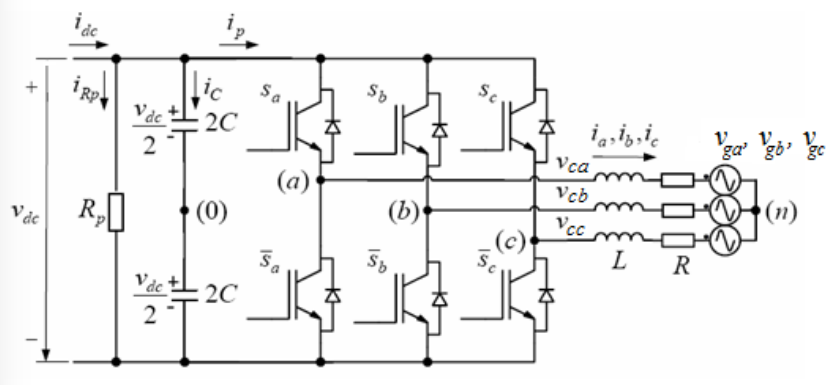
\includegraphics[width=.8\linewidth]{Images/FullConvFig.png}
    \caption{Three-phase inverter connected to the grid}
    \label{ModelFig}
  \end{figure}

  \begin{figure}[H]
    \centering
    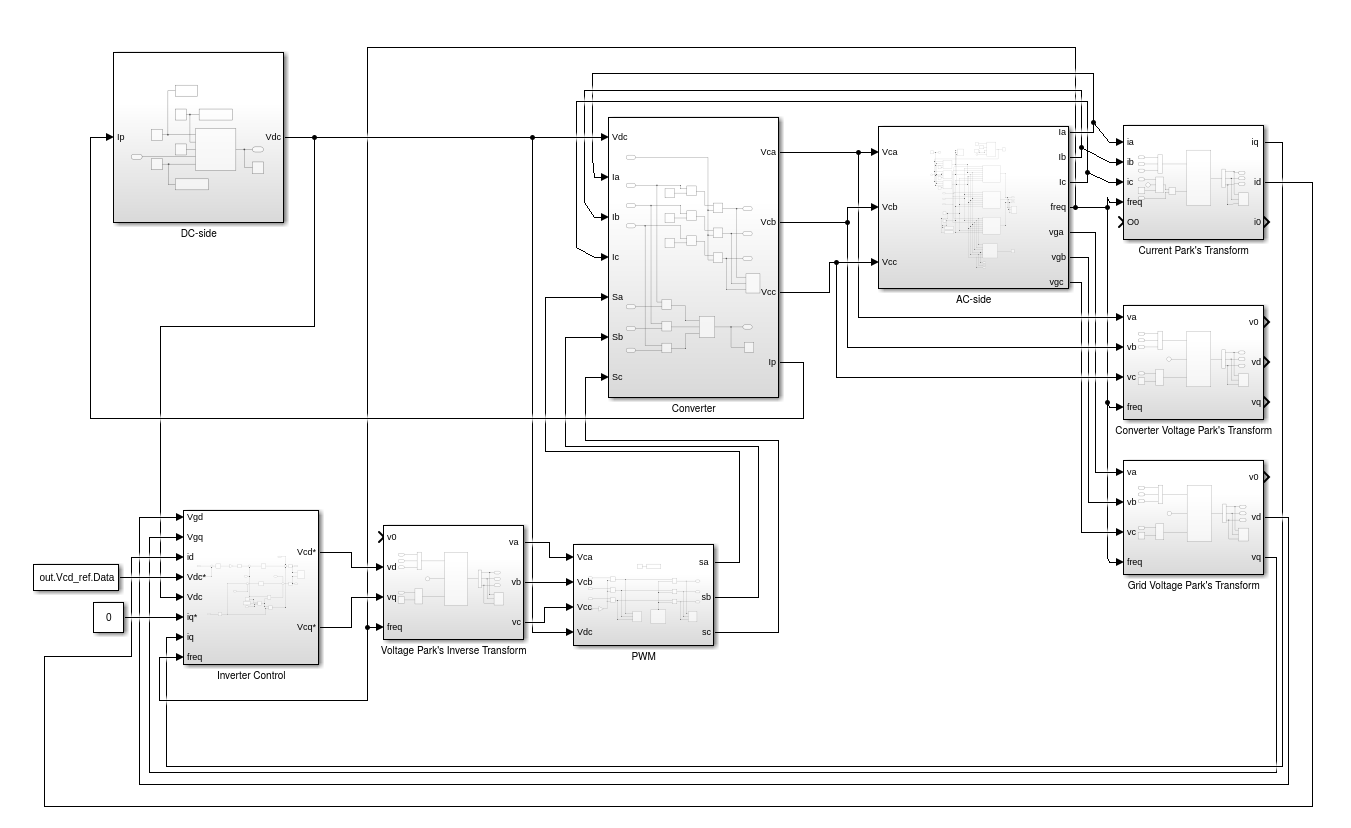
\includegraphics[width=.8\linewidth]{Images/S2_Model.png}
    \caption{Final model after the second lab session}
    \label{S1Model}
  \end{figure}


\chapter{Park's Transform}

  The model equations written in abc components from a non-linear system with differential equations have no analytical solution. Thus, it is necessary to change this equations by means of a transformation in order to remove the equations dependence on the mechanical angle to obtain a lineal system.\\
  We are transforming the abc components to dq components in a rotating frame of reference.\\

  \begin{figure}[H]
    \centering
    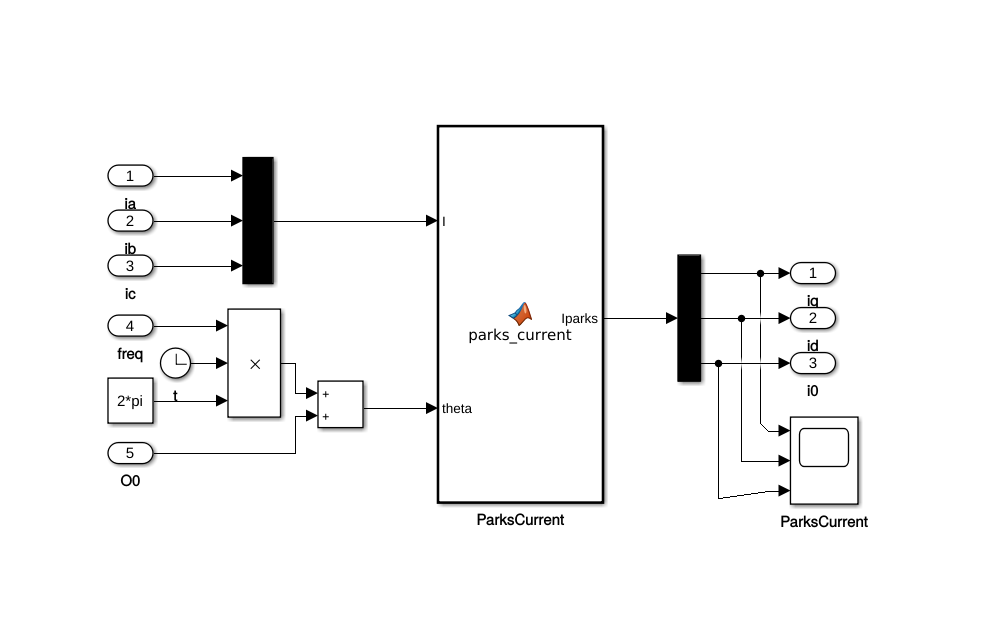
\includegraphics[width=.8\linewidth]{Images/ParksCurrentModel.png}
    \caption{Current Park's transform}
    \label{CurrentTransform}
  \end{figure}

  %Parks current transform code
  \begin{lstlisting}[language=Octave]
    function Iparks=parks_current(I,theta)
      Iparks=sqrt(2/3)*[cos(theta),cos(theta-120/180*pi),cos(theta+120/180*pi);
        sin(theta),sin(theta-120/180*pi),sin(theta+120/180*pi);
        .5,.5,.5]*I;
  \end{lstlisting}

  \begin{figure}[H]
    \centering
    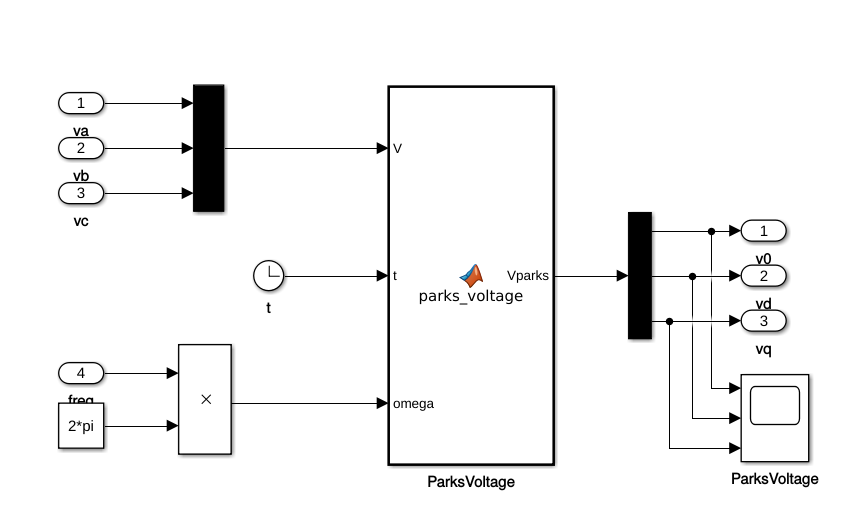
\includegraphics[width=.8\linewidth]{Images/ParksVoltage.png}
    \caption{Voltage Park's transform}
    \label{AC-side_eq}
  \end{figure}

  %Parks voltage transform code
  \begin{lstlisting}[language=Octave]
    function Vparks=parks_voltage(V,t,omega)
        Vparks=sqrt(2/3)*[1/sqrt(2),1/sqrt(2),1/sqrt(2);
            cos(omega*t),cos(omega*t-(2*pi)/(3)),cos(omega*t+(2*pi)/(3));
            -sin(omega*t),-sin(omega*t-(2*pi)/(3)),-sin(omega*t+(2*pi)/(3))]*V;
  \end{lstlisting}

  \begin{figure}[H]
    \centering
    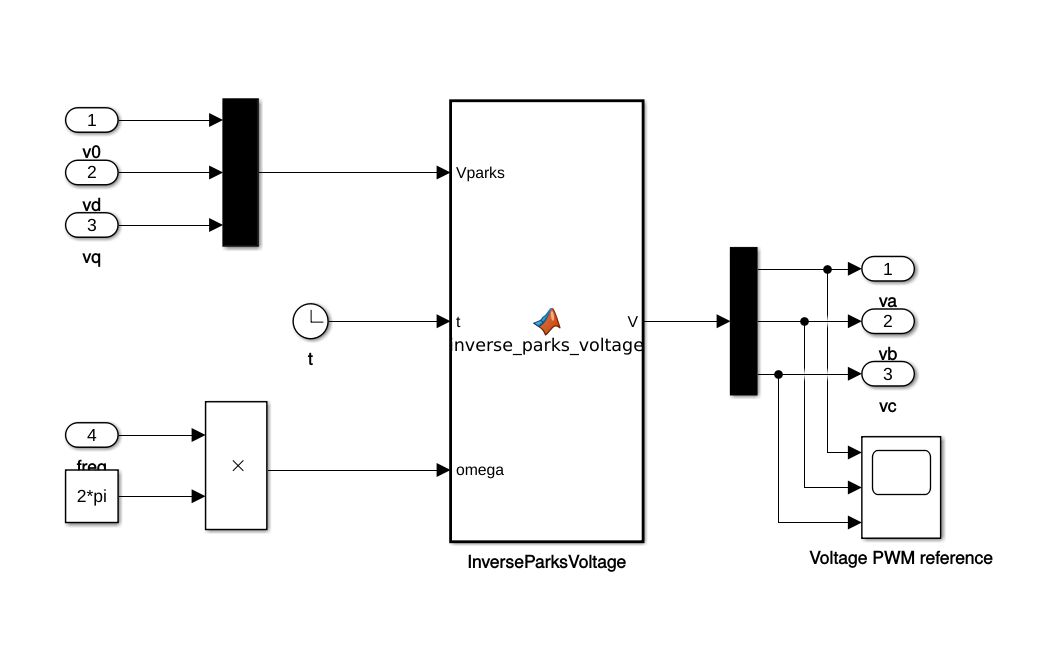
\includegraphics[width=.8\linewidth]{Images/InverseParksVoltage.png}
    \caption{Inverse voltage Park's transform}
    \label{AC-side_Simulink}
  \end{figure}

  %Parks inverse voltage transform code
  \begin{lstlisting}[language=Octave]
    function V=inverse_parks_voltage(Vparks,t,omega)
      V=sqrt(2/3)*[1/sqrt(2),1/sqrt(2),1/sqrt(2);
          cos(omega*t),cos(omega*t-(2*pi)/(3)),cos(omega*t+(2*pi)/(3));
          -sin(omega*t),-sin(omega*t-(2*pi)/(3)),-sin(omega*t+(2*pi)/(3))]\Vparks;
  \end{lstlisting}


\chapter{Modelling the PWM}

  The PWM genarator is used to trigger the IGBTs fiering in order to operate the inverter. The PWM is generated by comparing two signals scaled between -1 and 1, one of the signals is a sine wave obtained from the inverters dq voltages and the other is a triangular signal who's frequency is the same as the inverters switching frequency.\\

  \begin{figure}[H]
    \centering
    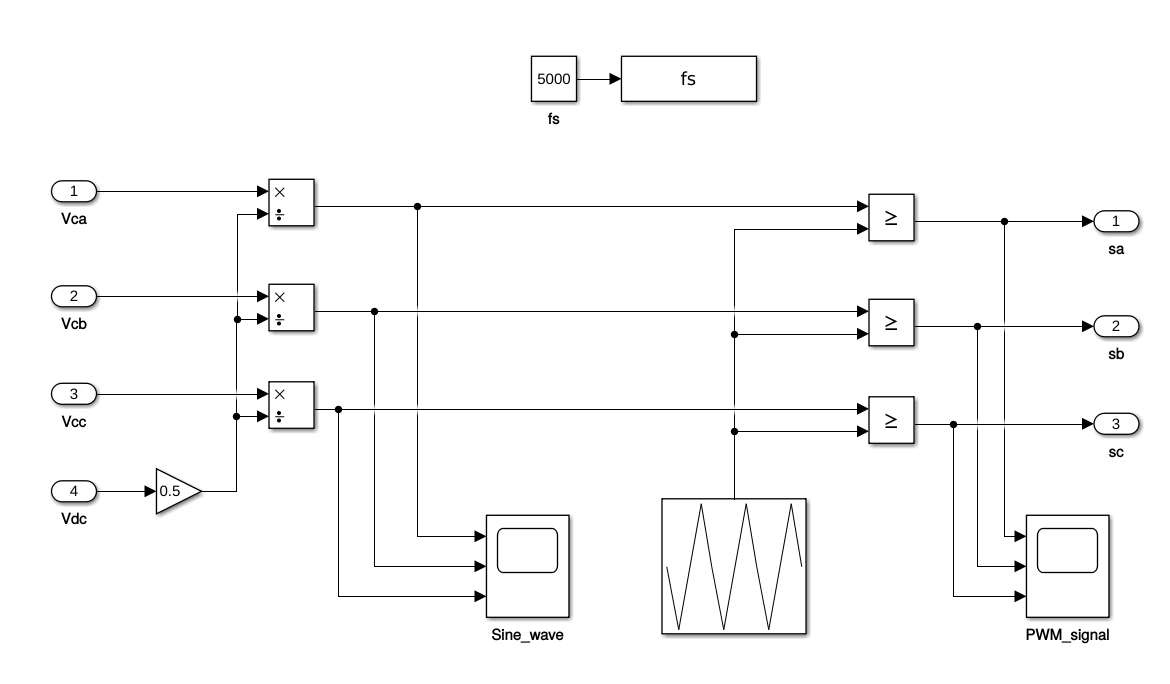
\includegraphics[width=1\linewidth]{Images/PWM.png}
    \caption{PWM generator}
    \label{PWM}
  \end{figure}


\chapter{Modelling the inverters control}

  Finally, the inverters control has also been modeled, however it is still not working as it should and will be fixed on the next session.

  \begin{figure}[H]
    \centering
    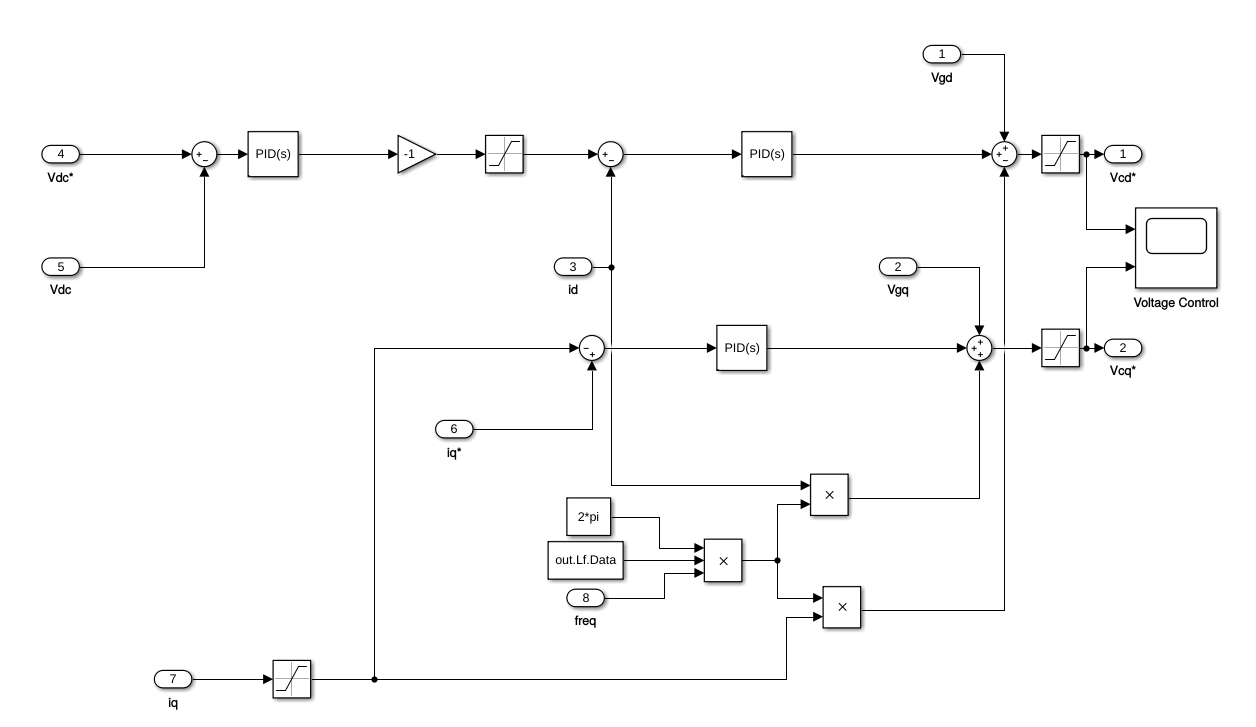
\includegraphics[width=1\linewidth]{Images/InverterControl.png}
    \caption{Inverter's control model}
    \label{Control}
  \end{figure}
